%%%%%%%%%%%%%%%%%%%%%%%%%%%%%%%%%%%%%%%%%
% Beamer Presentation
% LaTeX Template
% Version 1.0 (10/11/12)
%
% This template has been downloaded from:
% http://www.LaTeXTemplates.com
%
% License:
% CC BY-NC-SA 3.0 (http://creativecommons.org/licenses/by-nc-sa/3.0/)
%
%%%%%%%%%%%%%%%%%%%%%%%%%%%%%%%%%%%%%%%%%

\documentclass[t,usenames,dvipsnames]{beamer}
\mode<presentation> {
\usetheme{Boadilla}
\setbeamertemplate{navigation symbols}{} % To remove the navigation symbols from the bottom of all slides uncomment this line
}

\usepackage{graphicx} % Allows including images
\usepackage{booktabs} % Allows the use of \toprule, \midrule and \bottomrule in tables
\usepackage{amsmath}
\usepackage{amsthm}
\usepackage{cancel}
\usepackage{bussproofs}
\usepackage{proof}

\title[Graph minors]{Graph minors\\Robertson and Seymour's theorem in parameterized complexity}

\author{Narek Bojikian} % Your name
\institute[hu-berlin] % Your institution as it will appear on the bottom of every slide, may be shorthand to save space
{
Humboldt University of Berlin\\ % Your institution for the title page
\medskip
\textit{bojikian@informatik.hu-berlin.de} % Your email address
}
\date{\today} % Date, can be changed to a custom date

\begin{document}

\begin{frame}
\titlepage % Print the title page as the first slide
\end{frame}
\begin{frame} \frametitle{Graph minors}
	\begin{minipage}[t]{.59\linewidth}
	\begin{itemize}[<+->]
		\item Given graph $G$.
		\item $H$ is a minor of $G$,
			\begin{itemize}
				\item[] if $H$ results from $G$ by\\
					edge deletions and \textbf{contractions}.
			\end{itemize}
	\end{itemize}
	\end{minipage}
	\begin{minipage}[t]{.39\linewidth}
			\uncover<4->{Edge-contractions\\}%
			\only<4>{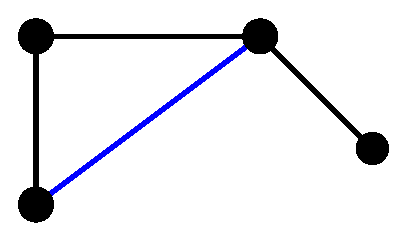
\includegraphics[width=0.9\linewidth]{contraction-0.eps}}%
			\only<5->{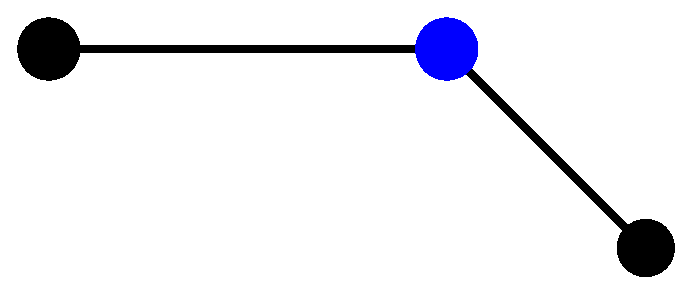
\includegraphics[width=0.9\linewidth]{contraction.eps}}%
	\end{minipage}
	\begin{itemize}[<+->]
		\item []
		\item []
		\item A graph $H$ is a minor of $G$ i.e. ``$H\leq_m G$'' iff\\
			there exists branch-set $V_h$ f.a. $h \in V(h)$ s.t.
			\begin{itemize}
				\item $G[V_h]$ is connected.
				\item for $g \neq h$ it holds $V_g \cap V_h = \emptyset$.
				\item for $\{g,h\} \in E(H)$, there exist $u_g \in V_g, u_h
					\in V_h$,\\
					s.t. $\{u_g, u_h\} \in E(G)$.
			\end{itemize}
		\item Are both definitions equivalent?
	\end{itemize}
\end{frame}
\begin{frame} \frametitle{Minor-closed classes}
	\begin{itemize}[<+->]
		\item Let $\mathcal{C}$ be some class of graphs.
		\item We call $\mathcal{C}$ minor-closed, if for all $G \in
			\mathcal{C}$\\
			\hspace{1cm}and $H\leq_m G$ it holds $H \in \mathcal{C}$.
			\\ \vspace{1cm}
		\item Examples:
			\begin{itemize}
				\item Forests.
				\item Graphs with vertex cover number $\leq k$.
				\item \textbf{Planar graphs}.
			\end{itemize}
	\end{itemize}
\end{frame}
\begin{frame} \frametitle{Planar Graphs}
	\begin{itemize}[<+->]
		\item Planar graphs are graphs\\
			\hspace{1cm}that can be \textbf{embedded} into the plane.
		\item An embedding is a corssing-free drawing.
		\item $K_5$ is not planar, but $K_4$ is.\\
			{
			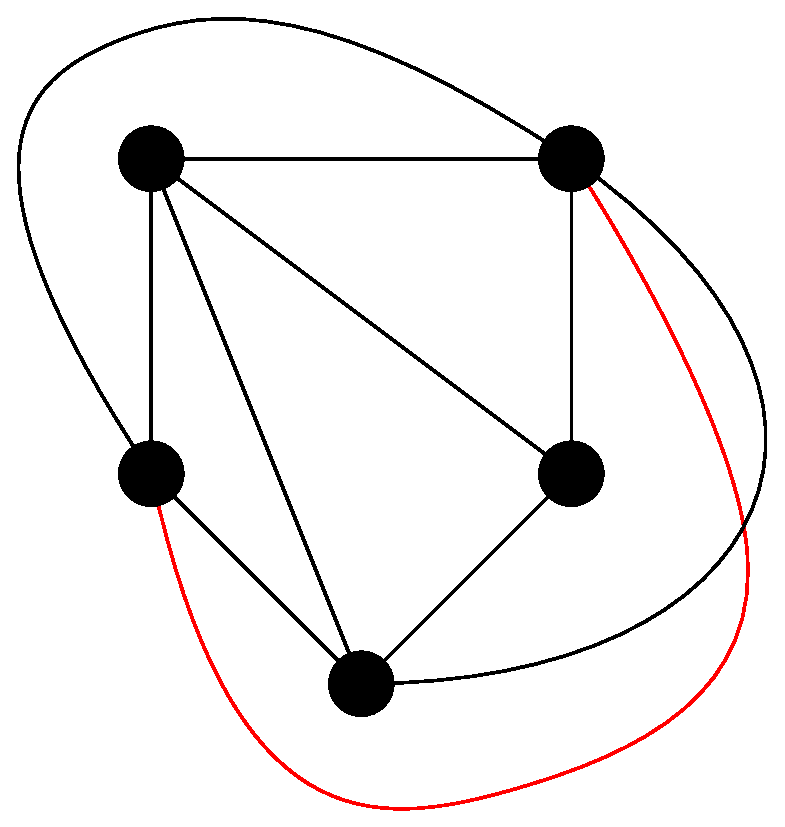
\includegraphics[width=0.3\linewidth]{k5.eps}
			\hspace{0.2\linewidth}
			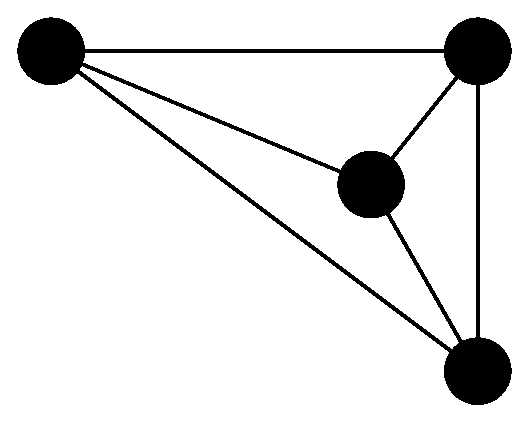
\includegraphics[width=0.3\linewidth]{k4.eps}
			}
		\item the class of planar graphs is minor-closed (why?).
			% -> we do not introduce crossings.
	\end{itemize}
\end{frame}
\begin{frame} \frametitle{Robertson and Seymour's Theorem}
	\begin{block}{Robertson and Seymour's Theorem [1]}
		The class of all graphs is well-quasi-ordered by the minor relation. That is in any
		infinite family of graphs, there are two graphs such that one is a minor of the
		other.
	\end{block}
	\uncover<2->{
	\begin{block} {Corollary} 
		For every minor-closed graph class $\mathcal{C}$, there exists a finite set
		$\operatorname{Forb}(\mathcal{C})$ of graphs with the following property: for every
		graph $G$, graph $G$ belongs to $\mathcal{C}$ if and only if ther edoes not exist a
		minor of $G$ that is isomorph to a member of $\operatorname{Forb}(\mathcal{C})$.
	\end{block}}
	\uncover<3->{
		\textbf{Proof sketch.}
	}
	
\end{frame}
\end{document} 
